\documentclass[]{article}
\usepackage{lmodern}
\usepackage{amssymb,amsmath}
\usepackage{ifxetex,ifluatex}
\usepackage{fixltx2e} % provides \textsubscript
\ifnum 0\ifxetex 1\fi\ifluatex 1\fi=0 % if pdftex
  \usepackage[T1]{fontenc}
  \usepackage[utf8]{inputenc}
\else % if luatex or xelatex
  \ifxetex
    \usepackage{mathspec}
  \else
    \usepackage{fontspec}
  \fi
  \defaultfontfeatures{Ligatures=TeX,Scale=MatchLowercase}
\fi
% use upquote if available, for straight quotes in verbatim environments
\IfFileExists{upquote.sty}{\usepackage{upquote}}{}
% use microtype if available
\IfFileExists{microtype.sty}{%
\usepackage{microtype}
\UseMicrotypeSet[protrusion]{basicmath} % disable protrusion for tt fonts
}{}
\usepackage[b5paper,tmargin=2.5cm,bmargin=2.5cm,lmargin=3.5cm,rmargin=2.5cm]{geometry}
\usepackage{hyperref}
\hypersetup{unicode=true,
            pdftitle={Big Brother Is Watching : Using Digital Surveillance Tools for Near Real-Time Mapping of the Risk of International Infectious Disease Spread},
            pdfauthor={Sangeeta Bhatia, Anne Cori and Pierre Nouvellet},
            pdfborder={0 0 0},
            breaklinks=true}
\urlstyle{same}  % don't use monospace font for urls
\usepackage{natbib}
\bibliographystyle{apalike}
\usepackage{longtable,booktabs}
\usepackage{graphicx,grffile}
\makeatletter
\def\maxwidth{\ifdim\Gin@nat@width>\linewidth\linewidth\else\Gin@nat@width\fi}
\def\maxheight{\ifdim\Gin@nat@height>\textheight\textheight\else\Gin@nat@height\fi}
\makeatother
% Scale images if necessary, so that they will not overflow the page
% margins by default, and it is still possible to overwrite the defaults
% using explicit options in \includegraphics[width, height, ...]{}
\setkeys{Gin}{width=\maxwidth,height=\maxheight,keepaspectratio}
\IfFileExists{parskip.sty}{%
\usepackage{parskip}
}{% else
\setlength{\parindent}{0pt}
\setlength{\parskip}{6pt plus 2pt minus 1pt}
}
\setlength{\emergencystretch}{3em}  % prevent overfull lines
\providecommand{\tightlist}{%
  \setlength{\itemsep}{0pt}\setlength{\parskip}{0pt}}
\setcounter{secnumdepth}{5}
% Redefines (sub)paragraphs to behave more like sections
\ifx\paragraph\undefined\else
\let\oldparagraph\paragraph
\renewcommand{\paragraph}[1]{\oldparagraph{#1}\mbox{}}
\fi
\ifx\subparagraph\undefined\else
\let\oldsubparagraph\subparagraph
\renewcommand{\subparagraph}[1]{\oldsubparagraph{#1}\mbox{}}
\fi

%%% Use protect on footnotes to avoid problems with footnotes in titles
\let\rmarkdownfootnote\footnote%
\def\footnote{\protect\rmarkdownfootnote}

%%% Change title format to be more compact
\usepackage{titling}

% Create subtitle command for use in maketitle
\newcommand{\subtitle}[1]{
  \posttitle{
    \begin{center}\large#1\end{center}
    }
}

\setlength{\droptitle}{-2em}
  \title{Big Brother Is Watching : Using Digital Surveillance Tools for Near
Real-Time Mapping of the Risk of International Infectious Disease Spread}
  \pretitle{\vspace{\droptitle}\centering\huge}
  \posttitle{\par}
  \author{Sangeeta Bhatia, Anne Cori and Pierre Nouvellet}
  \preauthor{\centering\large\emph}
  \postauthor{\par}
  \date{}
  \predate{}\postdate{}

\usepackage{booktabs}
\usepackage{amsthm}
\makeatletter
\def\thm@space@setup{%
  \thm@preskip=8pt plus 2pt minus 4pt
  \thm@postskip=\thm@preskip
}
\makeatother

\begin{document}
\maketitle

In our increasingly interconnected world, it is crucial to understand
the risk of an outbreak originating in one country/region and spreading
to the rest of the world. Rapid recognition and response to potential
pandemics and emerging diseases have become essential global health
priorities. Digital disease surveillance tools such as ProMed and
HealthMap have the potential to serve as important early warning systems
as well as complement the field surveillance data during an ongoing
outbreak. While there are a number of systems that carry out digital
disease surveillance, there is as yet a lack of tools that can compile
and analyse the generated data to produce easily understood actionable
reports. We present a flexible statistical model that uses different
streams of data (such as disease surveillance data, mobility data etc.)
for short-term incidence trend forecasting.\\
In validating the model using data collected by ProMED and HealthMap
during the 2014-2016 West African Ebola outbreak, we provide a realistic
appraisal of the strengths and limitations of such data in incidence
forecasting. We infer incidence trends at finer spatial scales from
aggregated data. Our work shows how the data from event based
surveillance systems (EBS) can complement the data collected from
traditional public health infrastructure. During an ongoing crisis,
combining data from different sources gives stakeholders a more complete
picture.

\section{Introduction}\label{introduction}

other tools that do similar stuff - EpiDMS \citep{liu2016epidms}
slightly old paper - authors curated news themselves!
\citep{chowell2016elucidating}

\section{Results}\label{results}

The raw data from ProMED is shown in Figure \ref{fig:hmraw}

\begin{figure}

{\centering 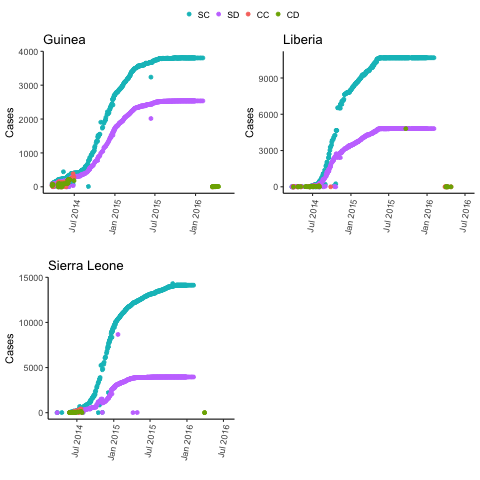
\includegraphics[width=6.67in]{figures/hmraw} 

}

\caption{Raw data from HealthMap}\label{fig:hmraw}
\end{figure}

\subsection{Cleaning ProMED/HealthMap data
feeds}\label{cleaning-promedhealthmap-data-feeds}

The data cleaning consists of the following steps : extracting the total
case counts as a sum of desired case categories, merging duplicate
alerts, removing data that made the cumulative case counts inconsistent
and finally, fill in the missing data using interpolation. Results at
each step pre-processing workflow for Sierra Leone are show in Figure
\ref{fig:hmclean}.

\begin{figure}

{\centering 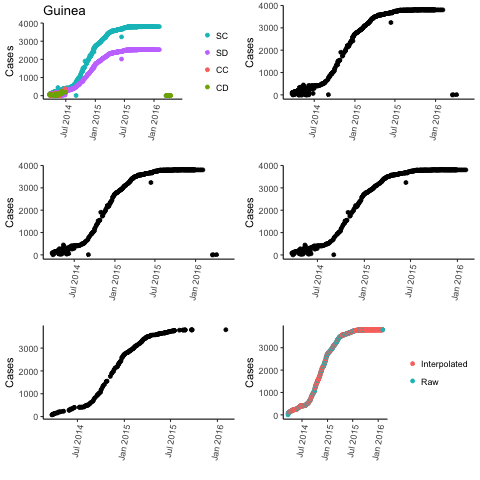
\includegraphics[width=6.67in]{figures/guinea} 

}

\caption{Data clean-up steps}\label{fig:hmclean}
\end{figure}

\subsection{Comparison of incidence trends from different
sources}\label{comparison-of-incidence-trends-from-different-sources}

\bibliography{bib/mriids.bib}


\end{document}
